\section{Clase 2}
\title[Circuitos Discretos]{Circuitos Discretos}
\subtitle{Clase 2: Repaso MOSFET}
\institute[]{Instituto Tecnológico de Costa Rica\\Escuela de Ingeniería Electrónica\\Circuitos Discretos}
\date{\theSemester}
\titlegraphic{
\includegraphics[height=8mm]{logoTEC.png}}

\begin{frame}[t]
\titlepage
\end{frame}

\begin{frame}[t]
    \frametitle{El transistor MOSFET}

    \begin{columns}
        \begin{column}{0.5\textwidth}
            El transistor MOSFET está formado por:
            \begin{itemize}
                \item Un sustrato (B)
                \item Dos regiones de difusión (D,G)
                \item Óxido de silicio (SiO\textsubscript{2})
                \item Polisilicio en compuerta (G)
                \item Contactos óhmicos en D,S
            \end{itemize}
        \end{column}
        \begin{column}{0.5\textwidth}
            \scalebox{0.9}{
                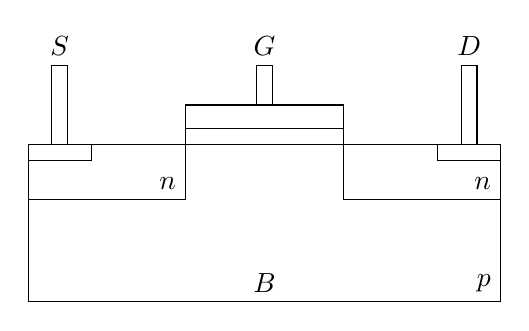
\begin{tikzpicture}
                    \draw (0,0) rectangle (6,2);        % sustrato
                    \draw (6,0) node[anchor=south east]{$p$};
                    \draw (0,1.3) rectangle (2,2);    % difusion S
                    \draw (2,1.3) node[anchor=south east]{$n$};
                    \draw (4,1.3) rectangle (6,2);    % difusion D
                    \draw (6,1.3) node[anchor=south east]{$n$};
                    %\draw (2,1.8) rectangle (4,2);      % canal
                    \draw (2,2) rectangle (4,2.2);      % SiO2
                    \draw (2,2.2) rectangle (4,2.5);    % Poly
                    \draw (0.3,2) rectangle (0.5,3);
                    \draw (5.5,2) rectangle (5.7,3);
                    \draw (2.9,2.5) rectangle (3.1,3);
                    \draw (3,3) node[anchor=south]{$G$};
                    \draw (0.4,3) node[anchor=south]{$S$};
                    \draw (5.6,3) node[anchor=south]{$D$};
                    \draw (3,0) node[anchor=south]{$B$};
                    \draw (0,2) rectangle (0.8,1.8);
                    \draw (5.2,2) rectangle (6,1.8);
                \end{tikzpicture}
            }        
        \end{column}
    \end{columns}
    
    \vspace{5mm}
    Las terminales del drenador y colector son intercambiables (siempre y cuando el sustrato no esté conectado a una de ellas).

    \begin{figure}[H]
        \centering
        \begin{circuitikz}
            \draw (0,0) node[nmos]{};
            \draw (2,0) node[pmos]{};
            \draw (4,0) node[nfet]{};
            \draw (6,0) node[pfet]{};
            \draw (8,0) node[nigfete]{};
            \draw (10,0) node[pigfete]{};
        \end{circuitikz}
        \caption{Símbolos del transistor MOSFET.}
        \label{mossymbols}
    \end{figure}
\end{frame}

\begin{frame}[t]
    \frametitle{El transistor MOSFET: Funcionamiento NMOS}

    Al aplicar tensión en la compuerta, se tienen los siguientes escenarios:

    \begin{columns}
        \begin{column}{0.5\textwidth}
            \centering

            \vspace{3mm}
            \textbf{Acumulación}

            \vspace{3mm}
            \begin{circuitikz}
                % MOS structure
                \draw (0,0) rectangle (3,1); % substrate
                \draw (0,0.7) rectangle (1,1); % source
                \draw (2,0.7) rectangle (3,1); % drain
                \draw (1,1) rectangle (2,1.1); % SiO2
                \draw (1,1.1) rectangle (2,1.3); % gate
                % labels for G, D, S, B
                \draw (0.5,0.7) node[anchor=north]{$S$};
                \draw (2.5,0.7) node[anchor=north]{$D$};
                \draw (1.5,0) node[anchor=south]{$B$};
                \draw (1.5,1.3) node[anchor=south]{$G$};
                % external circuitry
                \draw (1.1,1.3) -- (1.1,2);
                \draw (1.1,2) -- (-1,2);
                \draw (-1,0.15) to[vsource] (-1,2);
                \draw (0,0.85) -- (-0.3,0.85);
                \draw (-0.3,0.85) -- (-0.3,0.15);
                \draw (-1,0.15) -- (0,0.15);
                \draw (-1.5,1) node[anchor=east]{$V_{GS}$};
                % channel charge
                \draw (1.5,1) node[anchor=north,scale=0.7]{$++++$};
            \end{circuitikz}

            \vspace{3mm}
            \textbf{Agotamiento}

            \vspace{3mm}
            \begin{circuitikz}
                % MOS structure
                \draw (0,0) rectangle (3,1); % substrate
                \draw (0,0.7) rectangle (1,1); % source
                \draw (2,0.7) rectangle (3,1); % drain
                \draw (1,1) rectangle (2,1.1); % SiO2
                \draw (1,1.1) rectangle (2,1.3); % gate
                % labels for G, D, S, B
                \draw (0.5,0.7) node[anchor=north]{$S$};
                \draw (2.5,0.7) node[anchor=north]{$D$};
                \draw (1.5,0) node[anchor=south]{$B$};
                \draw (1.5,1.3) node[anchor=south]{$G$};
                % external circuitry
                \draw (1.1,1.3) -- (1.1,2);
                \draw (1.1,2) -- (-1,2);
                \draw (-1,2) to[vsource] (-1,0.15);
                \draw (0,0.85) -- (-0.3,0.85);
                \draw (-0.3,0.85) -- (-0.3,0.15);
                \draw (-1,0.15) -- (0,0.15);
                \draw (-1.5,1) node[anchor=east]{$V_{GS}$};
                % channel charge
                \draw (1.5,1) node[anchor=north,scale=0.7]{o o o o};
            \end{circuitikz}
        \end{column}
        \begin{column}{0.5\textwidth}
            \centering

            \vspace{3mm}
            \textbf{Inversión débil}
            
            \vspace{3mm}
            \begin{circuitikz}
                % MOS structure
                \draw (0,0) rectangle (3,1); % substrate
                \draw (0,0.7) rectangle (1,1); % source
                \draw (2,0.7) rectangle (3,1); % drain
                \draw (1,1) rectangle (2,1.1); % SiO2
                \draw (1,1.1) rectangle (2,1.3); % gate
                % labels for G, D, S, B
                \draw (0.5,0.7) node[anchor=north]{$S$};
                \draw (2.5,0.7) node[anchor=north]{$D$};
                \draw (1.5,0) node[anchor=south]{$B$};
                \draw (1.5,1.3) node[anchor=south]{$G$};
                % external circuitry
                \draw (1.1,1.3) -- (1.1,2);
                \draw (1.1,2) -- (-1,2);
                \draw (-1,2) to[vsource] (-1,0.15);
                \draw (0,0.85) -- (-0.3,0.85);
                \draw (-0.3,0.85) -- (-0.3,0.15);
                \draw (-1,0.15) -- (0,0.15);
                \draw (-1.5,1) node[anchor=east]{$V_{GS}$};
                % channel charge
                \draw (1.5,1) node[anchor=north,scale=0.7]{$-\ \ -$};
            \end{circuitikz}

            \vspace{3mm}
            \textbf{Inversión fuerte}
            
            \vspace{3mm}
            \begin{circuitikz}
                % MOS structure
                \draw (0,0) rectangle (3,1); % substrate
                \draw (0,0.7) rectangle (1,1); % source
                \draw (2,0.7) rectangle (3,1); % drain
                \draw (1,1) rectangle (2,1.1); % SiO2
                \draw (1,1.1) rectangle (2,1.3); % gate
                % labels for G, D, S, B
                \draw (0.5,0.7) node[anchor=north]{$S$};
                \draw (2.5,0.7) node[anchor=north]{$D$};
                \draw (1.5,0) node[anchor=south]{$B$};
                \draw (1.5,1.3) node[anchor=south]{$G$};
                % external circuitry
                \draw (1.1,1.3) -- (1.1,2);
                \draw (1.1,2) -- (-1,2);
                \draw (-1,2) to[vsource] (-1,0.15);
                \draw (0,0.85) -- (-0.3,0.85);
                \draw (-0.3,0.85) -- (-0.3,0.15);
                \draw (-1,0.15) -- (0,0.15);
                \draw (-1.5,1) node[anchor=east]{$V_{GS}$};
                % channel charge
                \draw (1.5,1) node[anchor=north,scale=0.7]{$----$};                
                \draw (1,0.7) -- (2,0.7);
            \end{circuitikz}
        \end{column}
    \end{columns}
\end{frame}

\begin{frame}[t]
    \frametitle{El transistor MOSFET: Curva de transferencia}

    \begin{multicols}{2}
        La \textbf{curva de transferencia} se mide al dejar $V_{DS}$ constante y modificar $V_{GS}$.

        \vspace{5mm}
        \begin{figure}[H]
            \begin{circuitikz}
                \draw (0,0) node[nmos](nmos1){};
                \draw (-2,0) to[battery1,l=$V_{GS}$] (-2,-1);
                \draw (-2,-1) node[ground]{};
                \draw (-2,0) -- (nmos1.gate);
                \draw (0,-1) node[ground]{};
                \draw (0,-1) -- (nmos1.source);
                \draw (2,1) to[V,l=$V_{DS}$] (2,-1);
                \draw (2,1) -- (0,1);
                \draw (0,1) -- (nmos1.drain);
                \draw (2,-1) node[ground]{};
                \draw [->] (-2.25,-0.75) -- (-1.75,-0.25);
            \end{circuitikz}
            %\caption{Circuito de medición de la curva de transferencia.}
            %\label{tfcircuit}
        \end{figure}
        
        \vspace{5mm}
        Esta curva está descrita por la ecuación:

        \[ I_D = \dfrac{1}{2}\mu_n C_{ox}' \dfrac{W}{L} (V_{GS}-V_{TH})^2 \]

        \newpage
        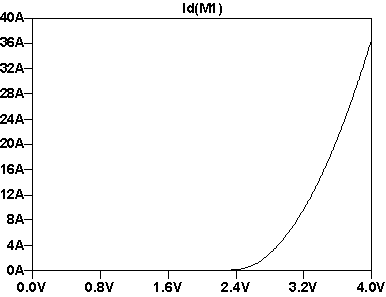
\includegraphics[width=5.5cm]{MOS_transfer.pdf}

    \end{multicols}
\end{frame}

\begin{frame}[t]
    \frametitle{El transistor MOSFET: Curva de salida}

    \begin{multicols}{2}
        La \textbf{curva de salida} se mide al mantener $V_{GS}$ constante y variar $V_{DS}$.

        \vspace{5mm}
        \begin{figure}[H]
            \begin{circuitikz}
                \draw (0,0) node[nmos](nmos1){};
                \draw (-2,0) to[V,l=$V_{GS}$] (-2,-1);
                \draw (-2,-1) node[ground]{};
                \draw (-2,0) -- (nmos1.gate);
                \draw (0,-1) node[ground]{};
                \draw (0,-1) -- (nmos1.source);
                \draw (2,1) to[battery1,l=$V_{DS}$] (2,-1);
                \draw (2,1) -- (0,1);
                \draw (0,1) -- (nmos1.drain);
                \draw (2,-1) node[ground]{};
                \draw [->] (1.75,-0.25) -- (2.25,0.25);
            \end{circuitikz}
            %\caption{Circuito de medición de la curva de salida.}
            %\label{tfcircuit2}
        \end{figure}

        \newpage
        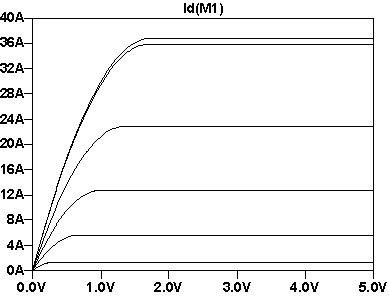
\includegraphics[width=5.5cm]{MOS_output.pdf}

    \end{multicols}

    En estas curvas se observa la diferencia entre la región de triodo y la región de saturación.

    \begin{itemize}
        \item Saturación: funcionamiento como fuente de corriente
        \item Triodo: funcionamiento como resistencia
    \end{itemize}
\end{frame}

\begin{frame}[t]
    \frametitle{El transistor MOSFET: Triodo ($V_{DS}<V_{GS}-V_{TH}$)}
    
    \centering
    \begin{figure}[H]
        \begin{tikzpicture}
            \draw (0,0) rectangle (6,2);        % sustrato
            \draw (0,1.3) rectangle (2,2);      % difusion S
            \draw (4,1.3) rectangle (6,2);      % difusion D
            \draw (2,1.4) -- (4,1.4);           % canal
            \draw (2,2) rectangle (4,2.2);      % SiO2
            \draw (2,2.2) rectangle (4,2.5);    % Poly
            % external circuitry
            \draw (-0.5,1.65) -- (0,1.65);
            \draw (-0.5,1.65) -- (-0.5,0.35);
            \draw (3,2.5) -- (3,3);
            \draw (3,3) -- (-2,3);
            \draw (-2,3) to[vsource,l=$V_{GS}$] (-2,0.35);
            \draw (-2,0.35) -- (0,0.35);
            \draw (5.6,2) -- (5.6,3);
            \draw (5.6,3) -- (8,3);
            \draw (8,3) to[vsource,l=$V_{DS}$] (8,0.35);
            \draw (8,0.35) -- (6,0.35);
            % labels for G, S, D, B
            \draw (3,3) node[anchor=south]{$G$};
            \draw (1,2) node[anchor=south]{$S$};
            \draw (5,2) node[anchor=south]{$D$};
            \draw (3,0) node[anchor=south]{$B$};
        \end{tikzpicture}
    \end{figure}

    \flushleft
    En la región del triodo, el canal está completamente formado.

    \vspace{3mm}
    La corriente es una función lineal de $V_{GS}$:

    \[ I_D = \mu_n C_{ox}' \dfrac{W}{L} \left((V_{GS}-V_{TH})V_{DS}+\dfrac{V_{DS}^2}{2}\right) \]

\end{frame}

\begin{frame}[t]
    \frametitle{El transistor MOSFET: Saturación ($V_{DS}>V_{GS}-V_{TH}$)}

    \centering
    \begin{figure}[H]
        \begin{tikzpicture}
            \draw (0,0) rectangle (6,2);        % sustrato
            \draw (0,1.3) rectangle (2,2);      % difusion S
            \draw (4,1.3) rectangle (6,2);      % difusion D
            \draw (2,1.4) -- (4,1.7);           % canal
            \draw (2,2) rectangle (4,2.2);      % SiO2
            \draw (2,2.2) rectangle (4,2.5);    % Poly
            % external circuitry
            \draw (-0.5,1.65) -- (0,1.65);
            \draw (-0.5,1.65) -- (-0.5,0.35);
            \draw (3,2.5) -- (3,3);
            \draw (3,3) -- (-2,3);
            \draw (-2,3) to[vsource,l=$V_{GS}$] (-2,0.35);
            \draw (-2,0.35) -- (0,0.35);
            \draw (5.6,2) -- (5.6,3);
            \draw (5.6,3) -- (8,3);
            \draw (8,3) to[vsource,l=$V_{DS}$] (8,0.35);
            \draw (8,0.35) -- (6,0.35);
            % labels for G, S, D, B
            \draw (3,3) node[anchor=south]{$G$};
            \draw (1,2) node[anchor=south]{$S$};
            \draw (5,2) node[anchor=south]{$D$};
            \draw (3,0) node[anchor=south]{$B$};
        \end{tikzpicture}
    \end{figure}

    \flushleft
    En la región de saturación, el canal se deforma.

    \vspace{3mm}
    La corriente es una función cuadrática de $V_{GS}$:

    \[ I_D = \dfrac{1}{2} \mu_n C_{ox}' \dfrac{W}{L} (V_{GS}-V_{TH})^2 \]

    \vspace{3mm}
    La tensión en el drenador es muy alta en comparación con la compuerta.

    \begin{itemize}
        \item DIBL: Drain-Induced Barrier Lowering
    \end{itemize}
    
\end{frame}

\begin{frame}[t]
    \frametitle{El transistor MOSFET: Modulación de Largo de Canal}

    \centering
    \begin{figure}[H]
        \begin{tikzpicture}
            \draw (0,0) rectangle (6,2);        % sustrato
            \draw (0,1.3) rectangle (2,2);      % difusion S
            \draw (4,1.3) rectangle (6,2);      % difusion D
            \draw (2,1.4) -- (3.6,2);           % canal
            \draw (2,2) rectangle (4,2.2);      % SiO2
            \draw (2,2.2) rectangle (4,2.5);    % Poly
            % external circuitry
            \draw (-0.5,1.65) -- (0,1.65);
            \draw (-0.5,1.65) -- (-0.5,0.35);
            \draw (3,2.5) -- (3,3);
            \draw (3,3) -- (-2,3);
            \draw (-2,3) to[vsource,l=$V_{GS}$] (-2,0.35);
            \draw (-2,0.35) -- (0,0.35);
            \draw (5.6,2) -- (5.6,3);
            \draw (5.6,3) -- (8,3);
            \draw (8,3) to[vsource,l=$V_{DS}$] (8,0.35);
            \draw (8,0.35) -- (6,0.35);
            % labels for G, S, D, B
            \draw (3,3) node[anchor=south]{$G$};
            \draw (1,2) node[anchor=south]{$S$};
            \draw (5,2) node[anchor=south]{$D$};
            \draw (3,0) node[anchor=south]{$B$};
        \end{tikzpicture}
    \end{figure}

    \flushleft
    El largo efectivo del canal disminuye conforme $V_{DS}$ aumenta.

    \[ I_D = \dfrac{1}{2} \mu_n C_{ox}' \dfrac{W}{L} (V_{GS}-V_{TH})^2 (1 + \lambda V_{DS}) \]

    En los alrededores del drenador, los electrones atraviesan una región de agotamiento.
\end{frame}

\begin{frame}[t]
    \frametitle{El transistor MOSFET: Subumbral ($V_{GS}<V_{TH}$)}

    En la región de subumbral, la tensión $V_{GS}$ es insuficiente para encender el transistor. La corriente sigue una característica de transferencia exponencial.

    \vspace{5mm}
    \begin{figure}[H]
        \centering
        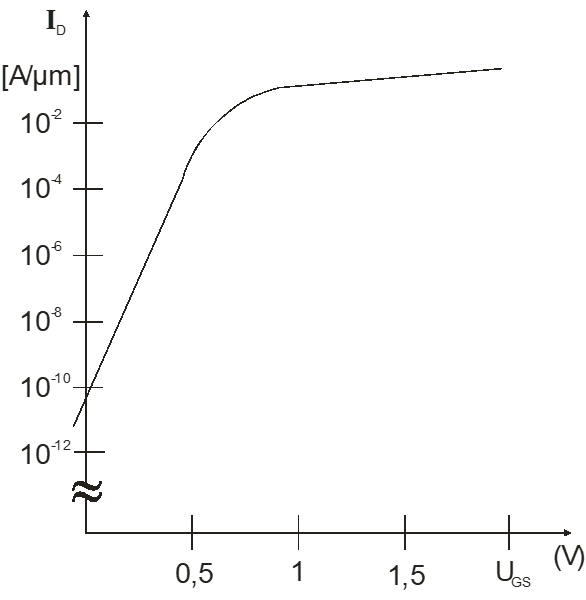
\includegraphics[width=5cm]{subthreshold.png}
        \caption{Curva de transferencia en la región de subumbral (Krautschneider, 2015).}
    \end{figure}
           
\end{frame}


\begin{frame}[t]
    \frametitle{El transistor MOSFET: Subumbral ($V_{GS}<V_{TH}$)}

    \begin{columns}
        \begin{column}{0.5\textwidth}
            La corriente en la región de subumbral:

            \[ I_D = I_{D0} \cdot e^{\dfrac{(V_{GS}-V_{TH})}{m \cdot V_t}} \]

            Se define la pendiente de subumbral:

            \[ S = \left( \dfrac{\partial \log_{10} I_D}{\partial V_{GS}} \right)^{-1} \]

            \[ S = \dfrac{\ln 10 \cdot kT \cdot m}{q} \]

            \[ S = \ln 10 \cdot V_t \cdot m \]

            \vspace{3mm}
            A T=300 K, $S\approx$ 80 ... 85 mV/dec

            A T=100 $^\circ$C, $S\approx$ 100 mV/dec
        \end{column}
        \begin{column}{0.5\textwidth}
            La corriente $I_{D0}$ es la corriente que fluye por el transistor cuando $V_{GS}=V_{TH}$.:

            \[ I_{D0} = I_D (V_{GS} = V_{TH}) \]

            \[ I_{D0} \approx 0.1\ \mu A \cdot \dfrac{W}{L} \]

            \vspace{3mm}
            La constante $m$ depende de la capacitancias de difusión y de la capacitancia del óxido:

            \[ m = \left( 1 + \dfrac{C_D}{C_{ox}} \right) \]
        \end{column}
    \end{columns}
\end{frame}


\begin{frame}[t]
    \frametitle{El transistor MOSFET: Efecto de Substrato}

    Al aplicar una tensión $V_{BS}$ entre el sustrato y la fuente, se vuelve más difícil formar un canal.

    \begin{itemize}
        \item La tensión de umbral (necesaria para establecer el canal) aumenta.    
    \end{itemize}

    \[ V_{TH} = V_{TH0} + \gamma ( \sqrt{2 \phi_B + V_{BS}} - \sqrt{2 \phi_B} ) \]

    \vspace{5mm}
    \begin{columns}
        \begin{column}{0.5\textwidth}
            \centering
            El coeficiente de \\ efecto de substrato:

            \[ \gamma = \dfrac{\sqrt{2q N_A \epsilon_{Si}}}{C_{ox}'} \]
        \end{column}
        \begin{column}{0.5\textwidth}
            \centering
            El potencial de \\ banda plana:

            \[ \phi_B = V_t \cdot \ln \left( \dfrac{N_A}{n_i} \right) \]
        \end{column}
    \end{columns}
\end{frame}

\begin{frame}[t]
    \frametitle{El transistor MOSFET: Polarización por Divisor de Tensión}

    \begin{columns}
        \begin{column}{0.5\textwidth}
            \begin{figure}[H]
                \centering
                \begin{tikzpicture}
                    \draw (0,2) node[nmos](nmos1){}
                    (-2,4) to[R,l=$R_1$] (-2,2){}
                    (-2,2) to[R,l=$R_2$] (-2,0){}
                    (-2,0) node[ground]{}
                    (-2,2) to[short] (nmos1.gate){}
                    (0,4) to[R, l=$R_D$] (nmos1.drain){}
                    (0,0) node[ground]{}
                    (0,0) to[short] (nmos1.source){}
                    (-2,5) to[short] (-2,4){}
                    (0,5) to[short] (0,4){}
                    (-2.5,5) to[short] (0.5,5)
                    (-1,5) node[anchor=south]{$V_{DD}$}
                    ;
                \end{tikzpicture}
            \end{figure}
        \end{column}
        \begin{column}{0.5\textwidth}
            La corriente en la compuerta es cero.

            \vspace{3mm}
            La tensión de compuerta es:

            \[ V_G = \dfrac{V_{DD} \times R_2}{R_1 + R_2} \]

            \[ V_G = V_{GS} \]

            \vspace{3mm}
            La corriente se obtiene directamente con la ecuación de saturación:

            \[ I_D = \dfrac{1}{2} \mu_n C_{ox}' \dfrac{W}{L} (V_{GS}-V_{TH})^2 \]

            \[ I_D = \dfrac{1}{2} \mu_n C_{ox}' \dfrac{W}{L} \left( \dfrac{V_{DD} \times R_2}{R_1 + R_2}-V_{TH} \right)^2 \]
        \end{column}
    \end{columns}
\end{frame}

\begin{frame}[t]
    \frametitle{El transistor MOSFET: Degeneración de Fuente}

    \begin{columns}
        \begin{column}{0.5\textwidth}
            \begin{figure}[H]
                \centering
                \begin{tikzpicture}
                    \draw (0,2) node[nmos](nmos1){}
                    (-2,4) to[R,l=$R_1$] (-2,2){}
                    (-2,2) to[R,l=$R_2$] (-2,0){}
                    (-2,0) node[ground]{}
                    (-2,2) to[short] (nmos1.gate){}
                    (0,4) to[R, l=$R_D$] (nmos1.drain){}
                    (0,0) node[ground]{}
                    (nmos1.source) to[R,l=$R_S$] (0,0){}
                    (-2,5) to[short] (-2,4){}
                    (0,5) to[short] (0,4){}
                    (-2.5,5) to[short] (0.5,5)
                    (-1,5) node[anchor=south]{$V_{DD}$}
                    ;
                \end{tikzpicture}
            \end{figure}
        \end{column}
        \begin{column}{0.5\textwidth}
            La tensión en la compuerta es:

            \[ V_G = \dfrac{V_{DD} \times R_2}{R_1 + R_2} \]

            La corriente $I_D$ se obtiene como:

            \[ I_D = \dfrac{V_S}{R_S} = \dfrac{V_G - V_{GS}}{R_S} \]

            Sin embargo, la tensión $V_{GS}$ depende de la corriente $I_D$:

            \[ V_{GS} = V_{TH} + \sqrt{\dfrac{2I_D}{\mu_n C_{ox}' \dfrac{W}{L}}} \]

            El sistema de ecuaciones se resuelve de tres posibles maneras: algebraicamente, iterando o por aproximación numérica con calcuadora.
        \end{column}
    \end{columns}
\end{frame}



\begin{frame}[t]
    \frametitle{El transistor MOSFET: Autopolarización}

    \begin{columns}
        \begin{column}{0.5\textwidth}
            \begin{figure}[H]
                \centering
                \begin{tikzpicture}
                    \draw (0,2) node[nmos](nmos1){}
                    (-3,3.5) to[short] (-3,2){}
                    (-3,2) to[short] (nmos1.gate){}
                    (0,6) to[R, l=$R_D$] (0,4){}
                    (0,4) to[short] (nmos1.drain){}
                    (0,1) node[ground]{}
                    (0,1) to[short] (nmos1.source){}
                    (-3,3.5) to[R,l=$R_G$] (0,3.5){}
                    (-0.5,6.5) to[short] (0.5,6.5)
                    (0,6.5) to[short] (0,6){}
                    (0,6.5) node[anchor=south]{$V_{DD}$}
                    ;
                \end{tikzpicture}
            \end{figure}        
        \end{column}
        \begin{column}{0.5\textwidth}
            En esta configuración:
            
            \begin{itemize}
                \item La corriente de compuerta es cero.
                \item La caída de tensión en $R_G$ es cero.
            \end{itemize}

            Por lo tanto, no importa el valor de la resistencia $R_G$. En la práctica se puede omitir y conectar directamente la compuerta al drenador.

            \[ V_{DD} = I_D R_D + V_{GS} \]

            \[ V_{DD} - V_{GS} = I_D R_D \]

            \[ I_D = \dfrac{V_{DD} - V_{GS}}{R_D} \]

            La tensión $V_{GS}$ es función de $I_D$.
        \end{column}
    \end{columns}
\end{frame}

\begin{frame}[t]
    \frametitle{El transistor MOSFET: Modelo de Pequeña Señal}

    \centering
    El modelo de peque\~{n}a se\~{n}al del transistor NMOS:

    \begin{circuitikz}
        \draw (0,2) -- (1,2);
        \draw (1,2) to[open,v=$v_{gs}$] (1,0);
        \draw (1,0) -- (5,0);
        \draw (3,2) to[cisource,l=$g_m v_{gs}$] (3,0);
        \draw (3,2) -- (6,2);
        \draw (5,2) to[R,l=$r_o$] (5,0);
        \draw (2,0) -- (2,-0.5);
        \draw (2,-0.5) node[anchor=north]{$S$};
        \draw (0,2) node[anchor=east]{$G$};
        \draw (6,2) node[anchor=west]{$D$};
    \end{circuitikz}

    El modelo de peque\~{n}a se\~{n}al del transistor PMOS:

    \begin{circuitikz}
        \draw (0,0) -- (1,0);
        \draw (1,2) to[open,v=$v_{sg}$] (1,0);
        \draw (1,2) -- (5,2);
        \draw (3,2) to[cisource,l=$g_m v_{sg}$] (3,0);
        \draw (3,0) -- (6,0);
        \draw (5,2) to[R,l=$r_o$] (5,0);
        \draw (2,2.5) -- (2,2);
        \draw (2,2.5) node[anchor=south]{$S$};
        \draw (0,0) node[anchor=east]{$G$};
        \draw (6,0) node[anchor=west]{$D$};
    \end{circuitikz}
\end{frame}

\begin{frame}[t]
    \frametitle{El transistor MOSFET: Transconductancia}

    \begin{columns}
        \begin{column}{0.5\textwidth}
            Por definición, la transconductancia es:

            \[ g_m = \left. \dfrac{\partial I_D}{\partial V_{GS}} \right|_Q \]
        
            Derivando la corriente de drenador:
        
            \[ g_m = \dfrac{\partial}{\partial V_{GS}} \left\{ \dfrac{1}{2} \mu_n C_{ox}' \dfrac{W}{L} (V_{GS}-V_{TH})^2 \right\} \]
        
            \[ \boxed{g_m = \mu_n C_{ox}' \dfrac{W}{L} (V_{GS}-V_{TH})} \]
            
            \vspace{3mm}
            Se define la tensión de sobrecarga:

            \[ V_{OV} = V_{GS} - V_{TH} \]

        \end{column}
        \begin{column}{0.5\textwidth}
            Otras formas de expresar la transconductancia:

            \[ g_m = \dfrac{2I_D}{V_{GS}-V_{TH}} \]

            \[ g_m = \sqrt{2 I_D \mu_n C_{ox}' \dfrac{W}{L} } \]

            \vspace{3mm}
            La impedancia de salida:

            \[ r_o = \dfrac{1}{\lambda I_D} \]

            \vfill
        \end{column}
    \end{columns}
\end{frame}

\begin{frame}[t]
    \frametitle{El transistor MOSFET: Impedancia desde el Drenador}

    \centering
    \begin{columns}
        \begin{column}{0.275\textwidth}
            \centering
            \scalebox{0.9}{
                \begin{circuitikz}
                    \draw [->] (-0.33,1.66) -- (-0.33,1);
                    \draw (-1,1.66) -- (-0.33,1.66);
                    \draw (-1,1.66) node[anchor=south]{$R_{out}$};
                    \draw (0,0) node[nmos](nmos1){};
                    \draw (-2,0) -- (nmos1.gate);
                    \draw (0,-1) -- (nmos1.source);
                    \draw (0,2) -- (nmos1.drain);
                    \draw (0,-1) node[ground]{};
                    \draw (-2,0) -- (-2,-1);
                    \draw (-2,-1) node[ground]{};
                \end{circuitikz}
            }
        \end{column}
        \begin{column}{0.725\textwidth}
            \centering
            \scalebox{0.9}{
                \begin{circuitikz}
                    \draw (-1,2) -- (-1,0);
                    \draw (-1,0) node[ground]{};
                    \draw (-1,2) -- (1,2);
                    \draw (1,2) to[open,v=$v_{gs}$] (1,0);
                    \draw (1,0) -- (5,0);
                    \draw (3,2) to[cisource,l=$g_m v_{gs}$] (3,0);
                    \draw (3,2) -- (7,2);
                    \draw (5,2) to[R,l=$r_o$] (5,0);
                    \draw (2,0) -- (2,-0.5);
                    \draw (2,-0.5) node[anchor=west]{$S$};
                    \draw (2,-0.5) node[ground]{};
                    \draw (0,2) node[anchor=south]{$G$};
                    \draw (6,2) node[anchor=south]{$D$};
                    \draw (7,2) to[V,l=$V_x$,i=$I_x$] (7,0);
                    \draw (7,0) node[ground]{};
                \end{circuitikz}
            }
        \end{column}
    \end{columns}

    \vspace{3mm}
    \flushleft
    \begin{columns}
        \begin{column}{0.5\textwidth}
            La impedancia desde la salida se mide al conectar una fuente de prueba $V_x$, y determinar la corriente $I_x$.

            \[ R_{out} = \dfrac{V_x}{I_x} \]

            \vspace{3mm}
            \begin{center}
                \textbf{La impedancia de salida se debe medir con la entrada a tierra.}
            \end{center}
        \end{column}
        \begin{column}{0.5\textwidth}
            \[ v_{gs} = 0 \]

            \[ I_x = \dfrac{V_x}{r_o} + g_m v_{gs} \]
    
            \[ \boxed{R_{out} = \dfrac{V_x}{I_x} = r_o} \]
        \end{column}
    \end{columns}
\end{frame}


\begin{frame}[t]
    \frametitle{El transistor MOSFET: Impedancia desde la Fuente}

    \centering
    \begin{columns}
        \begin{column}{0.3\textwidth}
            \centering
            \scalebox{0.9}{
                \begin{circuitikz}
                    \draw (0,0) node[nmos](nmos1){};
                    \draw (-2,0) -- (nmos1.gate);
                    \draw (0,-2) -- (nmos1.source);
                    \draw [->] (-0.33,-1.66) -- (-0.33,-1);
                    \draw (-1,-1.66) -- (-0.33,-1.66);
                    \draw (-1,-1.66) node[anchor=south]{$R_{out}$};
                    \draw (-2,0) node[ground]{};
                    \draw (nmos1.drain) node[ground,rotate=180]{};
                \end{circuitikz}
            }
        \end{column}
        \begin{column}{0.7\textwidth}
            \centering
            \scalebox{0.9}{
                \begin{circuitikz}
                    \draw (-1,2) -- (-1,0);
                    \draw (-1,0) node[ground]{};
                    \draw (-1,2) -- (1,2);
                    \draw (1,2) to[open,v=$v_{gs}$] (1,0);
                    \draw (1,0) -- (5,0);
                    \draw (3,2) to[cisource,l=$g_m v_{gs}$] (3,0);
                    \draw (3,2) -- (7,2);
                    \draw (5,2) to[R,l=$r_o$] (5,0);
                    \draw (2,0) to[V,l=$V_x$,i=$I_x$] (2,-2);
                    \draw (2,0) node[anchor=south]{$S$};
                    \draw (2,-2) node[ground]{};
                    \draw (0,2) node[anchor=south]{$G$};
                    \draw (6,2) node[anchor=south]{$D$};
                    \draw (7,2) node[ground]{};
                \end{circuitikz}
            }
        \end{column}
    \end{columns}

    \vspace{3mm}
    \flushleft
    Este circuito se analiza aplicando los siguientes métodos:

    \begin{itemize}
        \item LCK en el nodo de la fuente
        \item LVK en la malla desde la compuerta
    \end{itemize}

    \vspace{3mm}
    En general, aplicar una LCK en cada nodo del circuito, y una LVK por la base.
\end{frame}

\begin{frame}[t]
    \frametitle{El transistor MOSFET: Impedancia desde la Fuente}

    \begin{columns}
        \begin{column}{0.5\textwidth}
            La LVK por la compuerta:

            \[ 0 = v_{gs} + V_x \]

            \[ v_{gs} = -V_x \]

            \vspace{3mm}
            La LCK en la fuente:

            \[ I_x = \dfrac{V_x}{r_o} - g_m v_{gs} \]

            \vspace{3mm}
            Sustituyendo la LVK en la LCK:

            \[ I_x = \dfrac{V_x}{r_o} + g_m V_x \]
        \end{column}
        \begin{column}{0.5\textwidth}
            Factorizando la expresión anterior:

            \[ I_x = V_x \left( \dfrac{1}{r_o} + g_m \right) \]

            \vspace{3mm}
            Despejando la impedancia:

            \[ R_{out} = \dfrac{V_x}{I_x} = \dfrac{1}{\dfrac{1}{r_o} + g_m } \]

            \vspace{3mm}
            Observe que esto es el inverso de una suma de inversos:

            \[ \boxed{R_{out} = \dfrac{V_x}{I_x} = r_o \parallel \dfrac{1}{g_m}} \]

            \[ \boxed{R_{out} \approx 1/g_m} \]
        \end{column}
    \end{columns}

\end{frame}


\begin{frame}[t]
    \frametitle{El transistor MOSFET: Conexión como Diodo}

    \centering
    \begin{columns}
        \begin{column}{0.275\textwidth}
            \centering
            \scalebox{0.9}{
                \begin{circuitikz}
                    \draw (0,0) node[nmos](nmos1){};
                    \draw [->] (0.33,1.66) -- (0.33,1.33);
                    \draw (1,1.66) -- (0.33,1.66);
                    \draw (1,1.66) node[anchor=south]{$R_{out}$};
                    \draw (-1,0) -- (-1,1);
                    \draw (-1,0) -- (nmos1.gate);
                    \draw (-1,1) -- (0,1);
                    \draw (0,-1) -- (nmos1.source);
                    \draw (0,2) -- (nmos1.drain);
                    \draw (0,-1) node[ground]{};
                \end{circuitikz}
            }
        \end{column}
        \begin{column}{0.725\textwidth}
            \centering
            \scalebox{0.9}{
                \begin{circuitikz}
                    \draw (1,2) to[open,v=$v_{gs}$] (1,0);
                    \draw (1,0) -- (5,0);
                    \draw (3,2) to[cisource,l=$g_m v_{gs}$] (3,0);
                    \draw (1,2) -- (7,2);
                    \draw (5,2) to[R,l=$r_o$] (5,0);
                    \draw (2,0) -- (2,-0.5);
                    \draw (2,-0.5) node[anchor=west]{$S$};
                    \draw (2,-0.5) node[ground]{};
                    \draw (1,2) node[anchor=south]{$G$};
                    \draw (6,2) node[anchor=south]{$D$};
                    \draw (7,2) to[V,l=$V_x$,i=$I_x$] (7,0);
                    \draw (7,0) node[ground]{};
                \end{circuitikz}
            }
        \end{column}
    \end{columns}

    \begin{columns}
        \begin{column}{0.5\textwidth}
            La LVK por la compuerta:

            \[ V_x = v_{gs} \]

            \vspace{3mm}
            La LCK en el nodo G-D:

            \[ I_x = \dfrac{V_x}{r_o} + g_m v_{gs} \]
        \end{column}
        \begin{column}{0.5\textwidth}
            \vspace{3mm}
            Sustituyendo la LVK en la LCK:

            \[ I_x = \dfrac{V_x}{r_o} + g_m V_x \]

            \[ \boxed{R_{out} = \dfrac{V_x}{I_x} = r_o \parallel \dfrac{1}{g_m}}  \]

            \[ \boxed{R_{out} \approx 1/g_m} \]
        \end{column}
    \end{columns}
\end{frame}

